\section{Evaluation} \label{sec:eval}

We have evaluated our system on a 64-bit Dell server with 1GB memory
and a one-core Intel(R) Xeon(TM) CPU 2.80GH CPU. The OS, a Ubuntu
server 8.04 with kernel version 3.2.9, is installed on a Maxtor
7L250S0 3.5-inch SATA HDD. We used the same but another SATA HDD and
one Flash based SSD for MRIS store. The HDD is also a Maxtor 7L250S0
with a capacity of 250GB and a rotational speed of 7200 rpm.  The SSD
is an Intel SSDSA2CW300G3 2.5-inch with 300G capacity.  The code and
benchmark results are publicly available at
https://github.com/brianchenming/mris.

\subsection{Measure drives}
\label{sec:drives}

Firstly, we measured the two storage devices used in our benchmarks.
The results we got support our argument that Flash is good in random
I/O while HDD is not bad in sequential I/Os. We formated both devices
using Ext4. We remount devices before each benchmark to make sure that
all disk caches are dropped. The devices were measured using
Filebench~\cite{filebench-web}. Random read and write were measured
using Filebench built-in workloads \texttt{randomread} and
\texttt{randomwrite}; Sequential read and write were measured using
Filebench built-in workloads \texttt{singalstreamread} and
\texttt{singalstreamwrite}.

\begin{figure}[t]
\begin{centering}
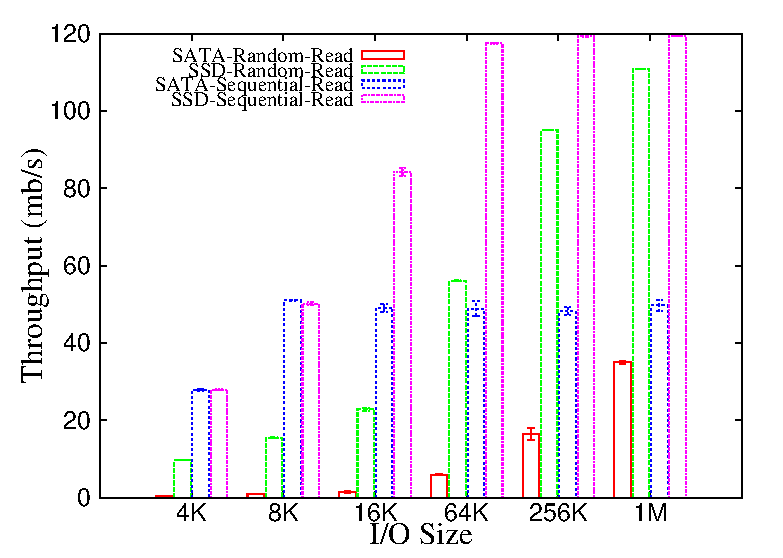
\epsfig{file=figures/ssd_vs_sata_read.eps,width=1.00\linewidth}
\caption{Read performance of SSD and HDD}
\label{fig:driveread}
\end{centering}
\end{figure}

The performance of read operations are presented in
Figure~\ref{fig:driveread}. All benchmarks are performed for 3 times,
and the standard deviation of the 3 runs are shown as error bar in the
figures. The results are stable and most error bars are imperceptible
or negligible. As we can see in Figure~\ref{fig:driveread}, SSD is
much better than that of HDD for random read for small I/O sizes. SSD
is 23.1$\times$ faster than HDD when I/O size is 4K, and 18.4$\times$
faster when I/O size is 8K. However, the speed advantage drops to
8.4$\times$ and 4.8$\times$ when the I/O size grows to 64K and 256K.
This is because disk head seek happens less frequently as I/O size
increases. Specifically, the HDD read throughput is 0.4mb/s with an
I/O size of 4K. This agrees with the 9ms average read time shown in
the HDD's specification.  

For sequential read, the most interesting observation is that HDD
provided the same throughput as SSD when I/O size is 4K and 8K. HDD
throughput stop grow after 8K, whereas SSD throughput grows until
256K. 8K and 256K are the points when HDD and SSD achieve their
respective maximum bandwidth.

\begin{figure}[t]
\begin{centering}
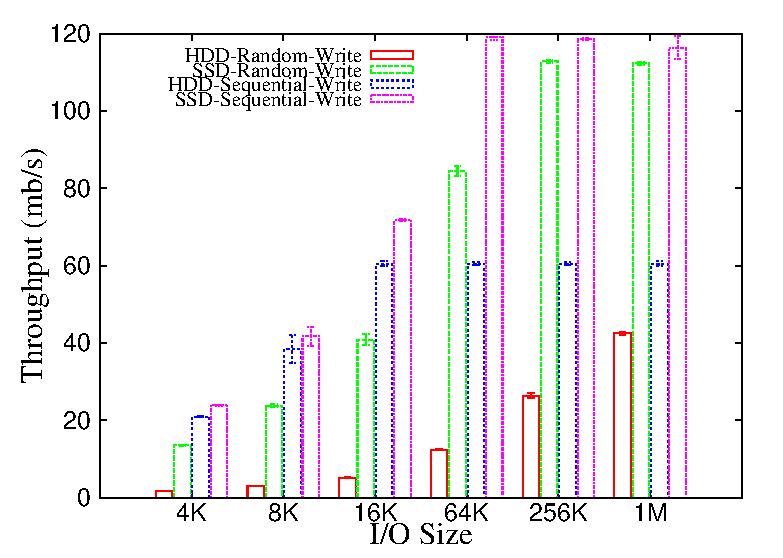
\epsfig{file=figures/ssd_vs_sata_write.eps,width=1.00\linewidth}
\caption{Write performance of SSD and HDD}
\label{fig:drivewrite}
\end{centering}
\end{figure}

The performances of write operations are presented in
Figure~\ref{fig:drivewrite}. They present similar trend as of read.
When I/O size is small (i.e. 4K, 8k, or 16k), SSD performs much better
than HDD for random write, but their performance have no significant
difference for sequential write. When I/O size becomes large,
throughput of both drives are capped by their maximum bandwidth.
However, we noticed that HDD performs better for write than for read.
This is because the HDD has a 16MB internal cache, which is more
helpful for write than for read. 

Above-mentioned results will serve as baselines of throughput for our
further benchmarking. They also validate our design premise that SSD
performs much better than HDD for random I/Os and HDD performs well
for sequential I/Os.

\subsection{Wikipedia Image Workload}

\begin{figure}[t]
\begin{centering}
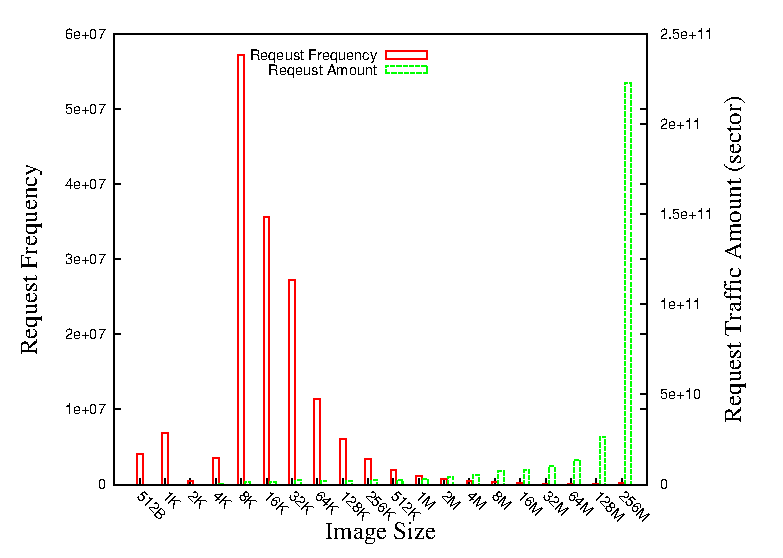
\epsfig{file=figures/wiki-image.eps,width=1.00\linewidth}
\caption{Image Requests to Wikipedia of January 2012}
\label{fig:wikiimage}
\end{centering}
\end{figure}

To study the size-tiered property in workloads, we analyzed the
requests of images made to Wikipedia site.  Wikipedia is the \#5
website in the world~\cite{wikipedia-web}, serving 492 million people
every month~\cite{wikimedia-foundation}. It can reflect workloads of
many large websites.

Figure~\ref{fig:wikiimage} presents the requests of images made in
January 2012. They are extracted from request log files from
http://dumps.wikimedia.org/other/pagecounts-raw/2012/2012-01/. We
extract requests of objects with a suffix of jpg, png, or gif, then
round up their sizes into power of 2. The frequency of images of
different sizes is counted and plotted in Figure~\ref{fig:wikiimage}.
All images larger than 256M is counted in the 256M bin. The first
observation from Figure~\ref{fig:wikiimage} is that the request image
of different sizes vary widely.  Particularly, images of sizes between
$(4, 64]$ KB are most popular. They sum to 81.58\% of the total number
of image requests. Moreover, 94.57\% of the requests are for images
smaller than or equal to 128KB. Despite the fact that small images
(smaller than 128KB) are the absolute majority in term of request
numbers, the traffic (size$\times$frequency) introduced by them is
just 2.96\% of the total. Although not all the requests make their way
to the storage layer because of memory cache (such as
Memcached~\cite{memcached}).  This salient size-tiered property of
requests still makes size-tiered storage a close match for
multi-resolution image workloads.

\subsection{MRIS Write}

%The drives were formatted using ext2, whereas fig:drivewrite was
%using ext4. This should not have happened. We need to redo one of the
%two sets of benchmarks in the future.

%TODO: specify that keys are not counted.

We now show micro benchmark results on simple workloads of sequential
and random write of multi-resolution images. Multi-resolution images
of the same content are often created from a common source. Therefore,
they are inserted into the image store at the same time. For example,
In Facebook's Haystack~\cite{beaver2010finding}, four resolutions,
thumbnail, small, medium, and large, are created from each image
uploaded by customers. As most images are in compressed format, we
emulate the workload of writing MRI by inserting groups of random
objects into MRIS with compression disabled. To be simple, each group
consists of two objects, both of which are random strings. One of the
two objects is 8KB large representing a small image, whereas the other
is 128KB large representing a large image. The SizeThreshold is set to
128KB, so that the large one will be stored in LargeSpace.

\begin{table}[tc]
{\centering \footnotesize
\begin{tabular}{c|c|c}
\hline 
  Setup & \multicolumn{2}{c}{Placement of Objects} \\ \cline{2-3}
   Name & Small (in SSTable) & Large (in LargeSpace) \\ \hline
  SSD & SSD & SSD \\
  Hybrid & SSD & HDD \\
  HDD & HDD & HDD \\ \hline 
\end{tabular}
 \caption{Setups For Benchmarking. The three setups differ in the
 places objects are stored.}
\label{tbl:setups}
}
\end{table}

Figure~\ref{fig:mriswrite} presents the results of the workload of
inserting 10,000 groups of objects into MRIS. We experimented the
workload on three different setups in Table~\ref{tbl:setups}. The
groups were inserted in random and sequential ways considering the
order of the key of objects. For ops/sec of random insertion, SSD is
28\% faster than HDD and Hybrid is 8\% faster than HDD. Considering
only SSD and HDD, the speedup of SSD is much lower than that shown in
Figure~\ref{fig:drivewrite}. This is because of the Memtable and the
log-structured feature of MRIS, which turns many random writes into
fewer large sequential write. It also explains how random writes
achieved a throughput of 23.9mb/sec even for HDD. As we can see in
Figure~\ref{fig:drivewrite}, SSD is only slightly faster than HDD
when it is for sequential write of 4K I/O size. Therefore, a slow
speedup of insertion is reasonable.

For sequential insertion, SSD is 26\% faster than HDD and Hybrid is
just 3\% faster than HDD. This is because sequential insertion causes
less compactions than random insertion, which reduce the overall
number of I/Os.  Compactions merge multiple sorted SSTable into one
larger sorted SSTable. When key/value pairs are inserted sequentially,
no merge is necessary because all SSTable have no overlapping keys.
This also explains why sequential insertion is significantly faster
than random insertion for all the three setups (41\%, 38\%, and 45\%
faster for SSD, Hybrid, and HDD). 

\NOTE{Ming}{I really should have recorded the number of compactions
happened during the benchmarking. I will probably do it in several
days.}

% How fdatasync determines which I/O size to use? We will have to
% double check the I/O size. LevelDB has an internal block size
% defaults to 4KB, but that is not necessarily the I/O size.

% LevelDB writes SSTable using mmap and fdatasync. It is better if we
% can get some basic drive benchmarks using mmap in the future.

Figure~\ref{fig:mriswrite} (b) also shows throughput in term of
mb/sec.  However, the speed-up ratio of mb/sec is almost identical to
that of ops/sec (differ in less than 0.1\%). This is what we are
expecting because the average size of an operation is the same among
all setups.

\begin{figure}[t]
  \centering
  \begin{minipage}[c]{\linewidth}
    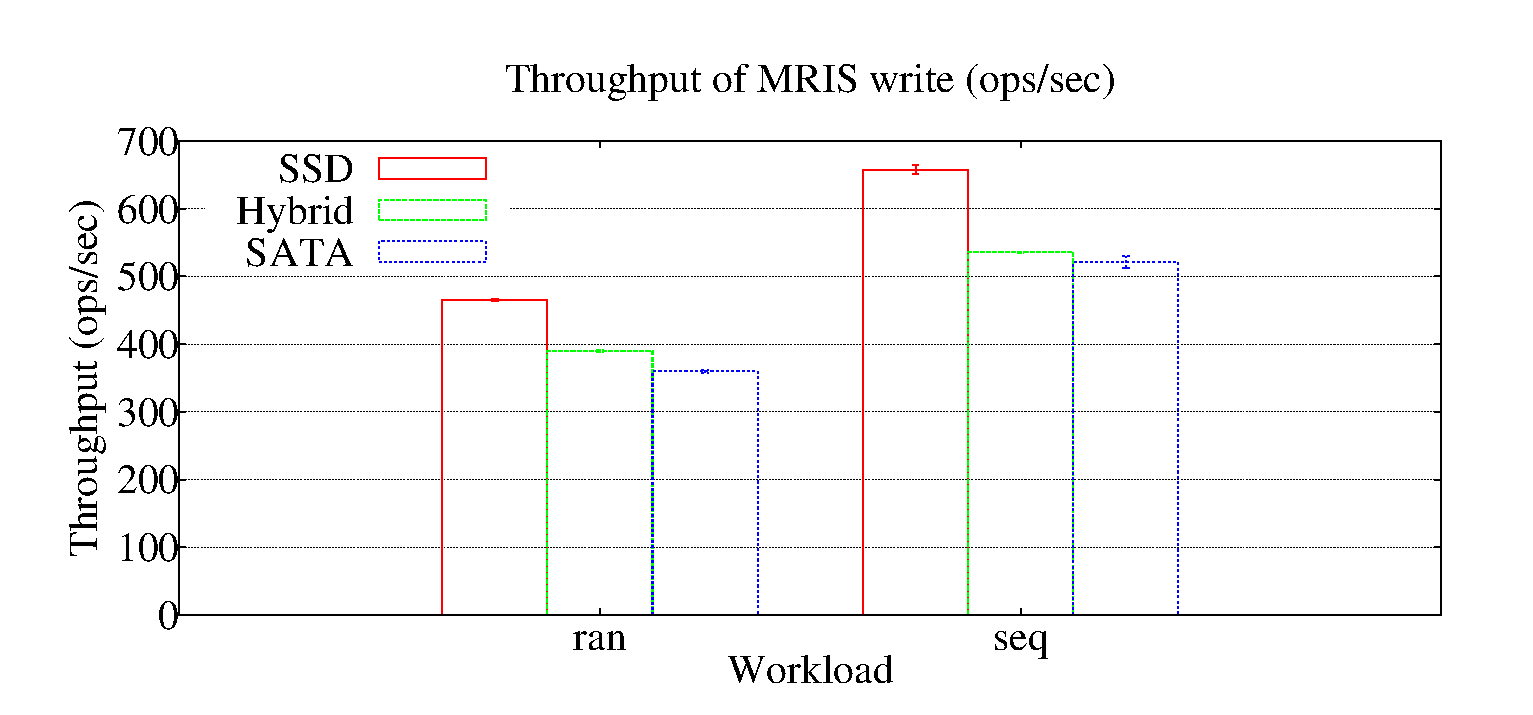
\epsfig{file=figures/mris-write-ops.eps,width=1.00\linewidth}
    \centerline{\footnotesize(a) Objects written per second}\medskip
  \end{minipage}
  \begin{minipage}[c]{\linewidth}
    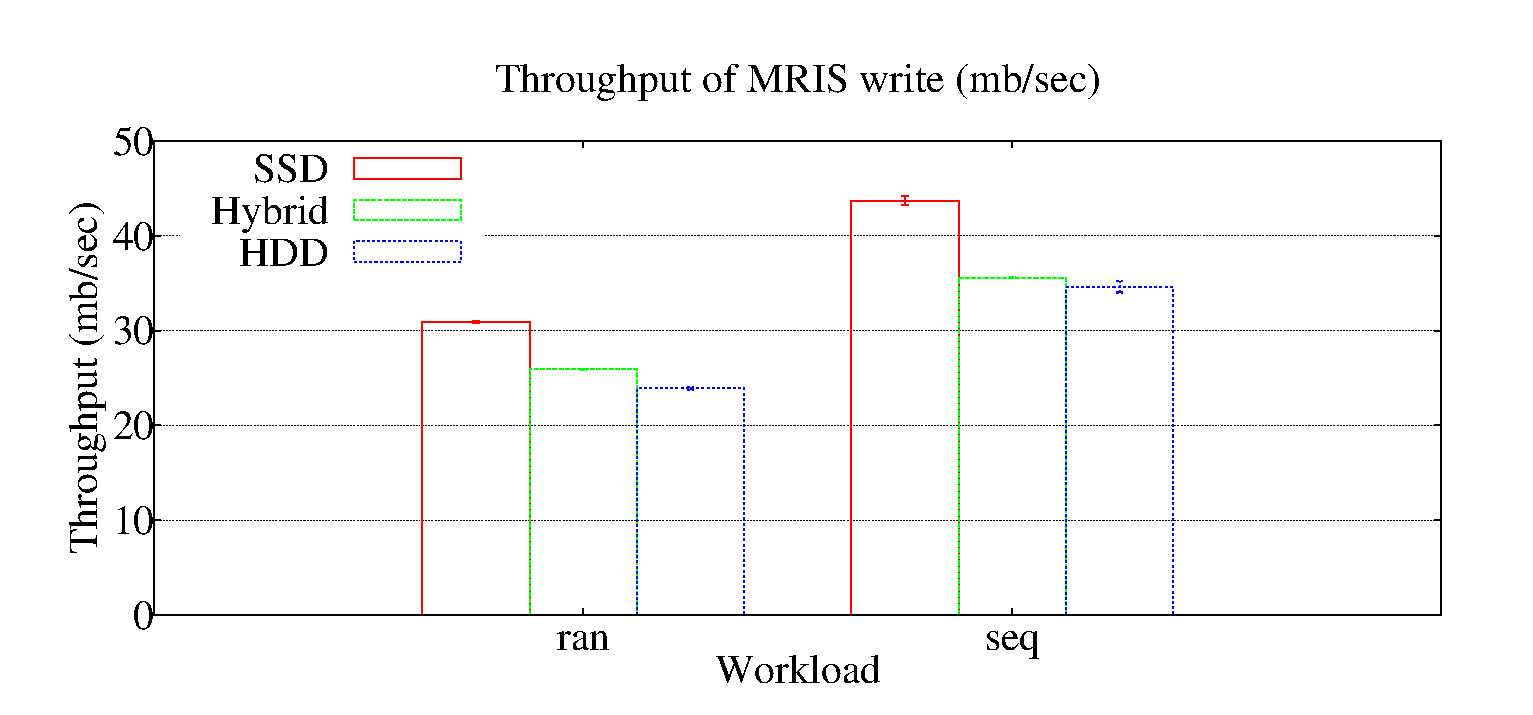
\epsfig{file=figures/mris-write-thput.eps,width=1.00\linewidth}
    \centerline{\footnotesize(b) MB written per second}\medskip
  \end{minipage}
  \caption{Write performance of MRIS.}
  \label{fig:mriswrite}
\end{figure}

\subsection{MRIS Read}

Log-structured key/value stores generally have high insertion
throughput, however, they also have to provide satisfactory lookup
performance.  We have developed workloads to evaluate the read
performance of MRIS.  One of the most interesting parameters in read
benchmarking is the ratio of reading small and large images. In
Facebook's workload~\cite{beaver2010finding}, the ratio of requests of
small and large images is around 17 (not considering thumbnails and
medium). In Wikipedia's workload, the ratio of requests of 8K-image
and 128K-image is around 9.5. In our benchmarks, we used different
ratios and performed workloads in all the three setups in
Table~\ref{tbl:setups}. Each benchmark randomly read 10,000 small
images from a database of 100,000 groups of images, and following
every $ratio$ reads of small images, one large version of the small
image is also read. For instance, one large image will be read after
every other read of small images when ratio is 2. This emulates the
common scenario that customers request large images once become
interested from the small ones.

\begin{figure}[t]
\begin{centering}
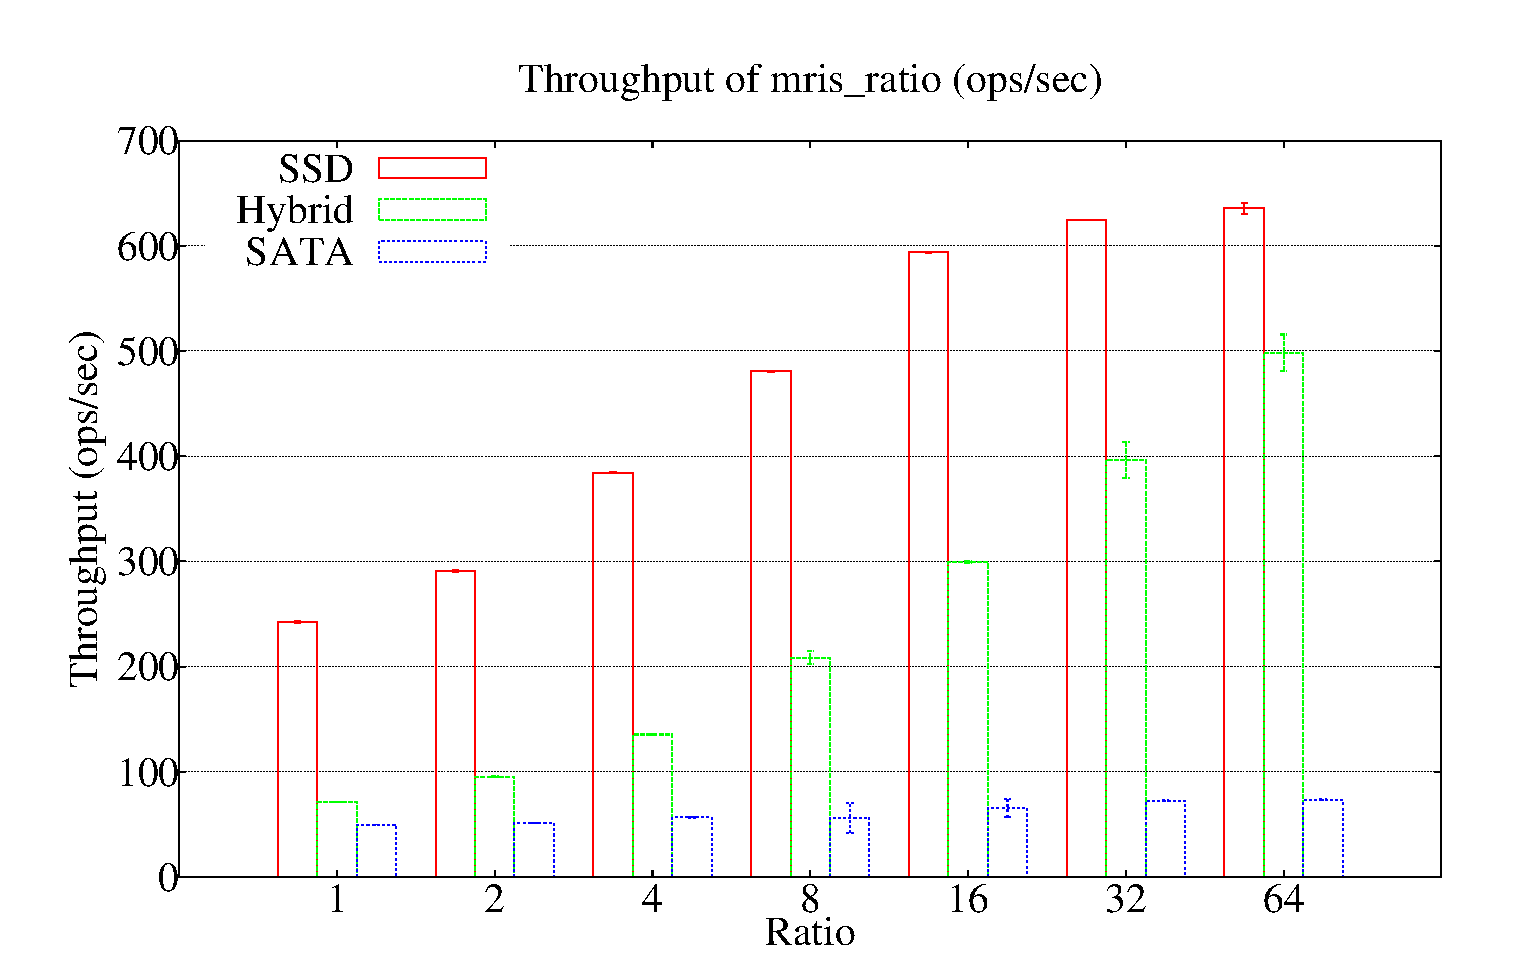
\epsfig{file=figures/mris_ratio_ops.eps,width=1.00\linewidth}
\caption{MRIS Read Performance (ops/sec). Each operation represents a
read of an image.}
\label{fig:mrisopssec}
\end{centering}
\end{figure}

Figure~\ref{fig:mrisopssec} presents the read throughput in term of
ops/sec. For all ratios, SSD shows the highest throughput among the
three setups, followed by Hybrid and then HDD. As shown in
Table~\ref{tbl:speedup}, the ops/sec of SSD is 3.89$\times$ to
7.64$\times$ faster than HDD. The speedup of SSD over HDD also grows
as ratio gets larger (except one point). This is because as the ratio
increases, the I/Os contain more small random reads, which exploits
more of SSD's superior random performance to HDD. Another interesting
observation is that the speedup of Hybrid over HDD grows rapidly from
0.44 to 5.78 as ratio increases.

\begin{table}[tc]
{\centering \footnotesize
\begin{tabular}{c|c|c|c|c|c|c|c}
\hline 
  Speedup & \multicolumn{7}{c}{Ratio} \\ \cline{2-8}
  over HDD & 1 & 2 & 4 & 8 & 16 & 32 & 64 \\ \hline
  SSD & 3.89 & 4.68 & 5.79 & 7.52 & 8.04 & 7.60 & 7.64  \\
  Hybrid & 0.44 & 0.86 & 1.39 & 2.69 & 3.56 & 4.46 & 5.78 \\ \hline
\end{tabular}
 \caption{Speedup of SSD and Hybrid over HDD (ops/sec).}
\label{tbl:speedup}
}
\end{table}

To help analyze the results, we use variables in
Table~\ref{tbl:variable} to represent the costs of involved read
operations in term of time. Then, ops/sec of SSD and HDD can be
expressed in (\ref{eqn:ssdops}) and (\ref{eqn:sataops}). 

\begin{equation}
\label{eqn:ssdops}
    1000000 \frac{ratio + 1}{t_{SF} * ratio + t_{LF}}
\end{equation}

\begin{equation}
\label{eqn:sataops}
    1000000 \frac{ratio + 1}{t_{SH} * ratio + t_{LH}}
\end{equation}

Using linear regression, we estimated the values of the variables
(also shown in Table~\ref{tbl:variable}) from our benchmark data.
Approximately, the ops/sec of Hybrid can be expressed in
(\ref{eqn:hybridops}).

\begin{equation}
\label{eqn:hybridops}
    1000000 \frac{ratio + 1}{t_{SF} * ratio + t_{LH}}
\end{equation}

\begin{table}[tc]
{\centering \footnotesize
\begin{tabular}{c|c|c}
\hline 
  Read Type & Flash SSD & SATA HDD \\ \hline
  Small Image & $t_{SF} = 1482$ & $t_{SH} = 13238$ \\ 
  Large Image & $t_{LF} = 6542$ & $t_{LH} = 37599$ \\ \hline
\end{tabular}
 \caption{Costs of read operations in time ($\mu$s). For instance,
$t_{SF}$ is the time of reading a Small image from the Flash SSD.}
\label{tbl:variable}
}
\end{table}

Use (\ref{eqn:hybridops}) and the values in Table~\ref{tbl:variable},
we can predict the ops/sec of Hybrid. The results, together with
measured ops/sec in our benchmarks, are presented in
Figure~\ref{fig:opspred}. We can see that the measured ops/sec
matches the shape of the predicted ops/sec. Moreover, the measured
ops/sec are all slightly higher than the predicted counterparts.

% TODO: measure the prediction accuracy with quantitative metrics

\begin{figure}[t]
\begin{centering}
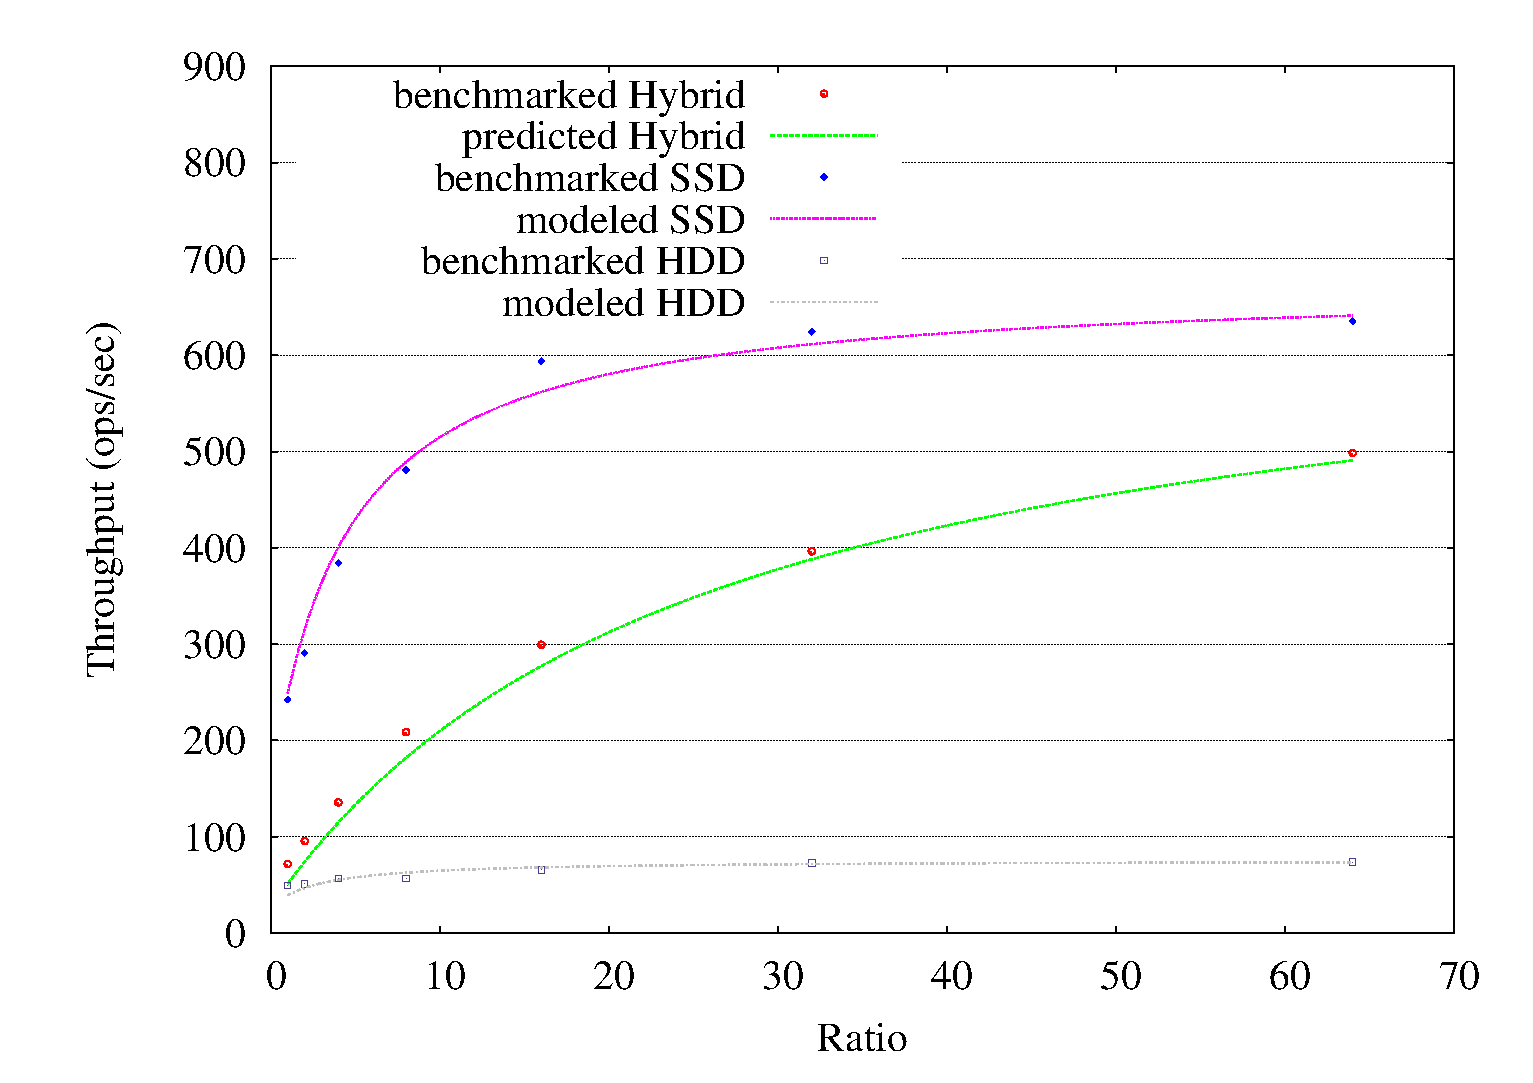
\epsfig{file=figures/ratio_ops_predict.eps,width=\linewidth}
\caption{Modeled and benchmarked performance (ops/sec).}
\label{fig:opspred}
\end{centering}
\end{figure}

For the same workloads, the throughputs in term of mb/sec are
presented in Figure~\ref{fig:mrismbsec}. Different from the results of
ops/sec, mb/sec is decreasing as ratio increases for both SSD and
HDD. This is because more of the operations are reads of small images
when ratio is large. As we can see in (\ref{eqn:opsize}), the average
size of an operation is a monotonically decreasing function of ratio
where $large = 128\mbox{KB}$ and $small = 8\mbox{KB}$ are the sizes of
large and small images respectively.

\begin{equation}
\label{eqn:opsize}
\begin{array}{r@{\quad=\quad}l}
  \mbox{avg\_op\_size} & \frac{ratio * small + large}{ratio + 1} \\
   & \mbox{small} + \frac{large - small}{ratio + 1} 
\end{array}
\end{equation}

\begin{figure}[t]
\begin{centering}
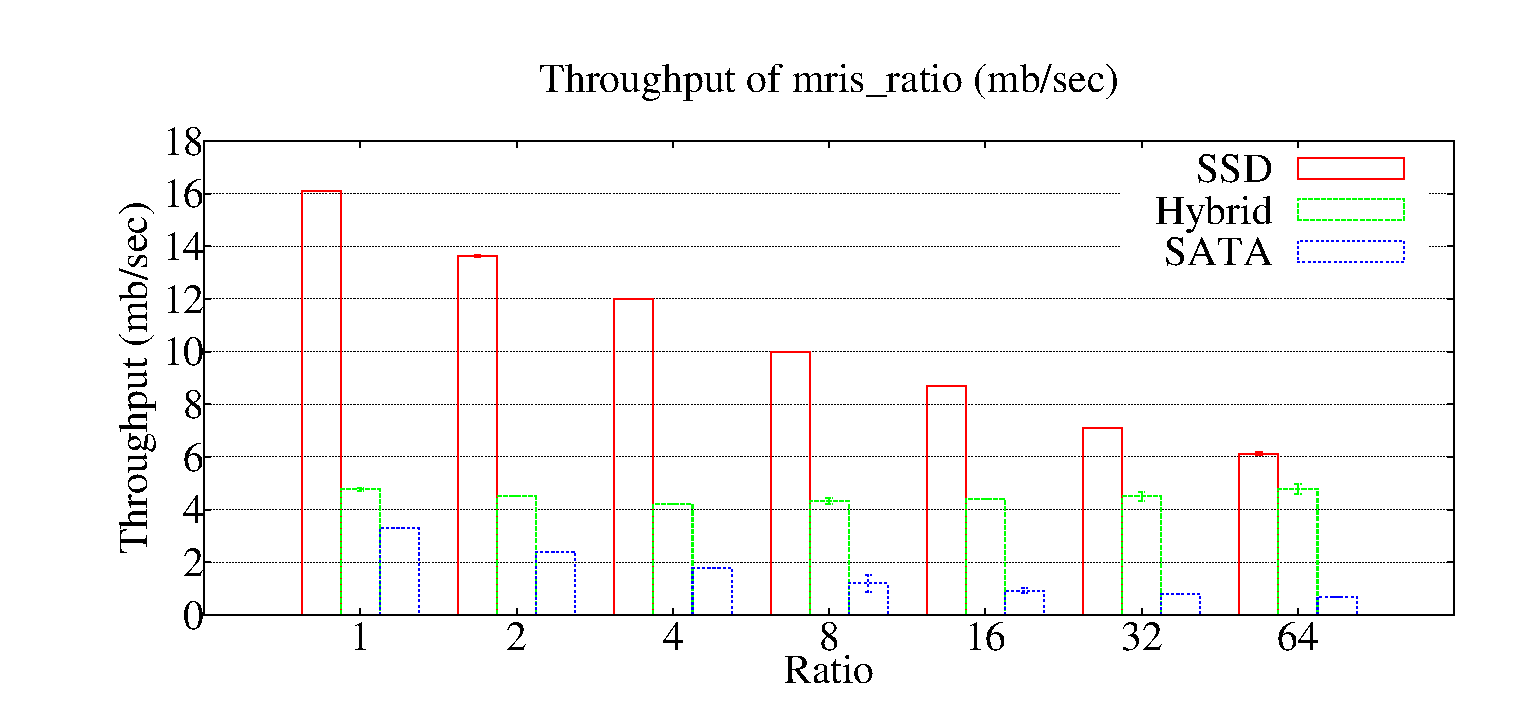
\epsfig{file=figures/mris_ratio_thput.eps,width=1.00\linewidth}
\caption{MRIS Read Performance (mb/sec).}
\label{fig:mrismbsec}
\end{centering}
\end{figure}

However, for Hybrid, the throughputs in Figure~\ref{fig:mrismbsec} are
relatively stable. Derived from (\ref{eqn:hybridops}), the mb/sec of
Hybrid can be expressed in

\begin{equation}
\label{eqn:hybridthput}
    1000000 \frac{ratio * small + large}{t_{SF} * ratio + t_{LH}} .
\end{equation}

Similarly, we can predict the mb/sec of SSD and HDD. The predicted
mb/sec results, along with the benchmarked mb/sec results, are
presented in Figure~\ref{fig:thputpred}. We observed that there exists
significant discrepancy in Hybrid's mb/sec results when ratio is
small. This is because the average operation size is large when ratio
is small, as we can see from (\ref{eqn:opsize}). The distances between
predicted ops/sec and benchmarked ops/sec of small ratios, in
Figure~\ref{fig:mrisopssec}, are magnified when turned to mb/sec by
multiplying the average operation size.

\begin{figure}[t]
\begin{centering}
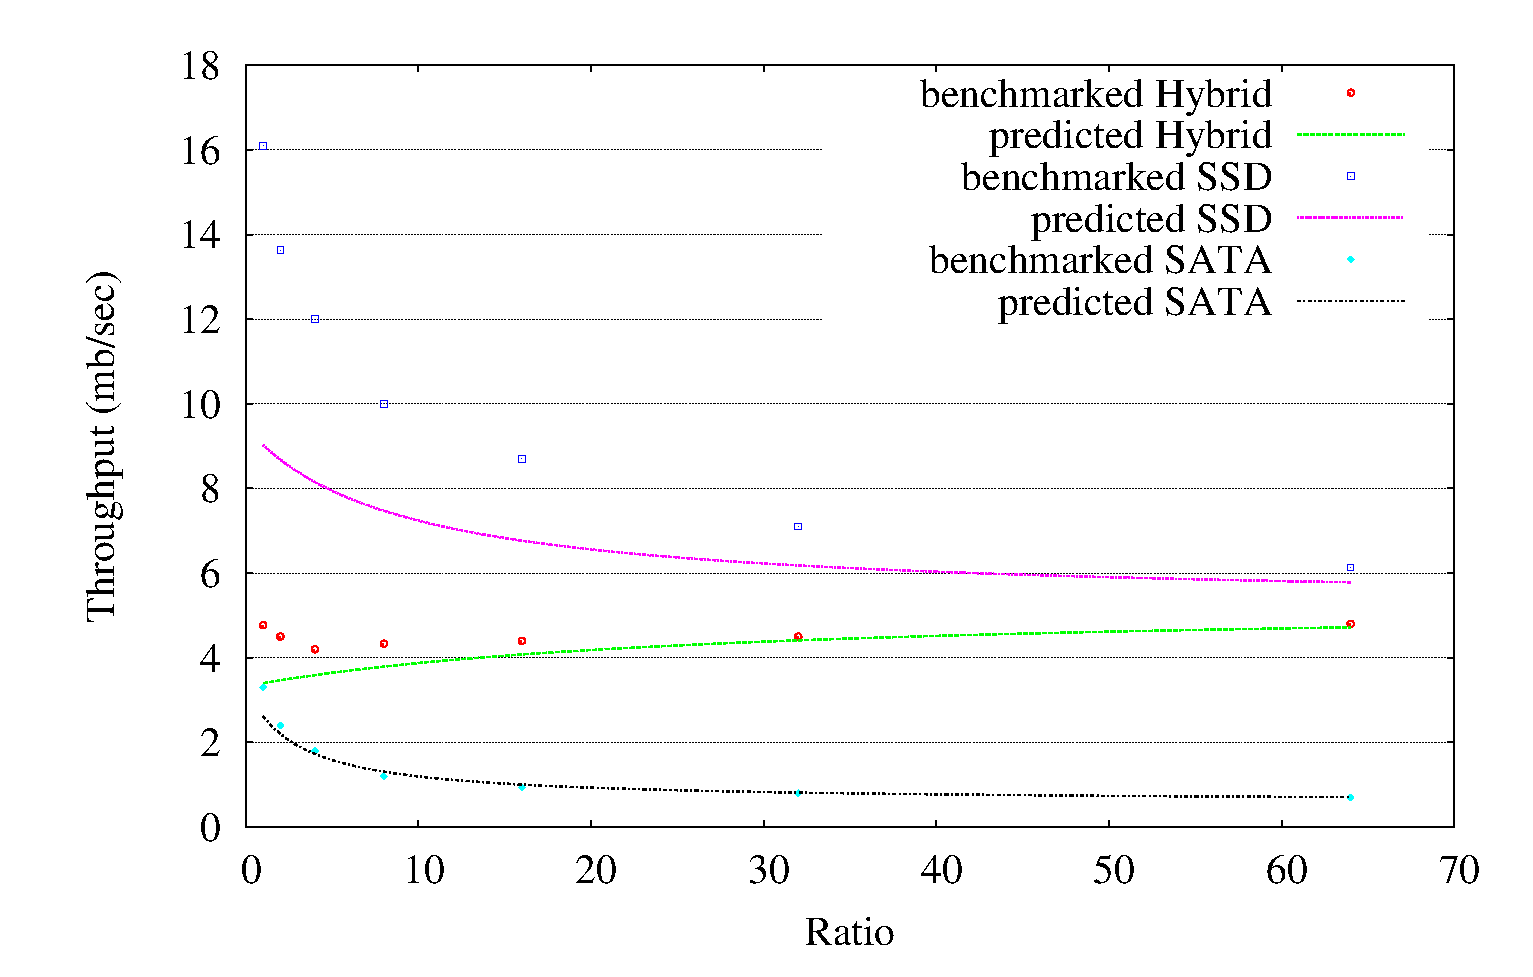
\epsfig{file=figures/ratio_thput_predict.eps,width=\linewidth}
\caption{Predicted and benchmarked read performance (mb/sec).}
\label{fig:thputpred}
\end{centering}
\end{figure}

As presented in Table~\ref{tbl:spdupmb}, Hybrid improves HDD's mb/sec
throughput by at least 45\%. The improvement grows to as high as
5.86$\times$ when ratio is 64.  Specifically, the speedup is
2.61$\times$ and 3.73$\times$ when ratio is 8 and 16, which
approximate to the ratios in the workloads of Wikipedia and Facebook.

\begin{table}[tc]
{\centering \footnotesize
\begin{tabular}{c|c|c|c|c|c|c|c}
\hline 
  Speedup & \multicolumn{7}{c}{Ratio} \\ \cline{2-8}
  over HDD & 1 & 2 & 4 & 8 & 16 & 32 & 64 \\ \hline
  SSD & 3.88 & 4.68 & 5.67 & 7.33 & 8.35 & 7.87 & 7.76 \\
  Hybrid & 0.45 & 0.88 & 1.33 & 2.61 & 3.73 & 4.62 & 5.86 \\ \hline
\end{tabular}
 \caption{Speedup of SSD and Hybrid over HDD (mb/sec).}
\label{tbl:spdupmb}
}
\end{table}

%\NOTE{Ming}{TODO: consitify terms, such as images and objects, HDD and
%SATA}

We have also measured the throughput (mb/sec) went to each drive using
\texttt{iostat}. The results are shown in Figure~\ref{fig:mrisiostat}.
We observed that the throughput reported by iostat is much larger than
that in Figure~\ref{fig:mrisopssec}. Three factors contribute to the
extra throughput: 1) the read-ahead in the filesystem, 2) extra read
of filesystem metadata, and 3) extra read of database metadata.
However, it is interesting to notice that the data read from SSD for
the SSD setup is quite stable even when ratio varies dramatically.
This is something we need to further investigate.

\begin{figure}[t]
\begin{centering}
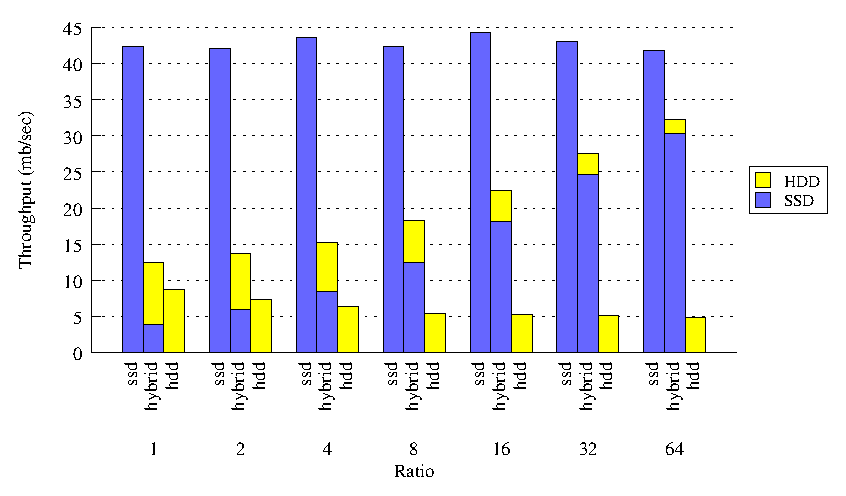
\epsfig{file=figures/mris_ratio_iostat_thput.eps,width=1.00\linewidth}
\caption{MRIS Read Performance (mb/sec) by iostat}
\label{fig:mrisiostat}
\end{centering}
\end{figure}

%%%%%%%%%%%%%%%%%%%%%%%%%%%%%%%%%%%%%%%%%%%%%%%%%%%%%%%%%%%%%%%%%%%%%%%%%%%%%%
%% For Emacs:
% Local variables:
% fill-column: 70
% End:
%%%%%%%%%%%%%%%%%%%%%%%%%%%%%%%%%%%%%%%%%%%%%%%%%%%%%%%%%%%%%%%%%%%%%%%%%%%%%%
%% For Vim:
% vim:textwidth=70 noai nocin nosi
%%%%%%%%%%%%%%%%%%%%%%%%%%%%%%%%%%%%%%%%%%%%%%%%%%%%%%%%%%%%%%%%%%%%%%%%%%%%%%
% LocalWords:  
